%
% eindiomensional.tex -- Lösung der eindimensionalen DGL
%
% (c) 2021 Prof Dr Andreas Müller, OST Ostschweizer Fachhochschule
% Erstellt durch Roy Seitz
%
% !TeX spellcheck = de_CH
\bgroup

\begin{frame}[t]
  \setlength{\abovedisplayskip}{5pt}
  \setlength{\belowdisplayskip}{5pt}
  \frametitle{Beispiel $\sin x$}
  \vspace{-20pt}
  %\onslide<+->
  \begin{block}{Taylor-Approximationen von $\sin x$}
    \begin{align*}
      p_n(x)
      &= 
      \uncover<1->{0}
      \uncover<2->{+ x}
      \uncover<3->{+ 0 \frac{x^2}{2!}}
      \uncover<4->{- 1 \frac{x^3}{3!}}
      \uncover<5->{+ 0 \frac{x^4}{4!}}
      \uncover<6->{+ 1 \frac{x^5}{5!}}
      \uncover<7->{+ \ldots}
      \uncover<8->{
        = \sum_{k=0}^{n/2} (-1)^{2k + 1}\frac{x^{2k+1}}{(2k+1)!}
      }
    \end{align*}
  \end{block}
  \begin{center}
    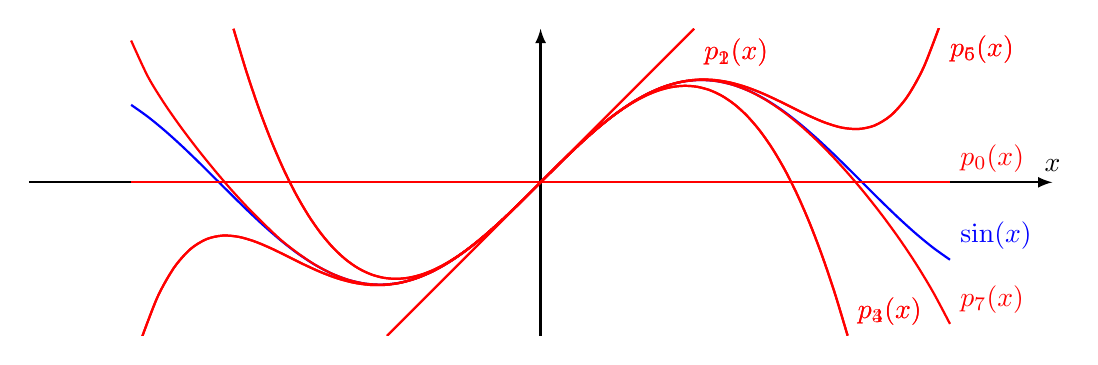
\begin{tikzpicture}[>=latex,thick,scale=1.3]
      \draw[->] (-5.0, 0.0) -- (5.0,0.0) coordinate[label=$x$];
      \draw[->] ( 0.0,-1.5) -- (0.0,1.5);
      \clip (-5,-1.5) rectangle (5,1.5);
      \draw[domain=-4:4, samples=50, smooth, blue]
      plot ({\x}, {sin(180/3.1415968*\x)})
      node[above right] {$\sin(x)$};
      \uncover<1>{
        \draw[domain=-4:4, samples=2, smooth, red]
        plot ({\x}, {0})
        node[above right] {$p_0(x)$};}
      \uncover<2>{
        \draw[domain=-1.5:1.5, samples=2, smooth, red]
        plot ({\x}, {\x})
        node[below right] {$p_1(x)$};}
      \uncover<3>{
        \draw[domain=-1.5:1.5, samples=2, smooth, red]
        plot ({\x}, {\x})
        node[below right] {$p_2(x)$};}
      \uncover<4>{
        \draw[domain=-3:3, samples=50, smooth, red]
        plot ({\x}, {\x - \x*\x*\x/6})
        node[above right] {$p_3(x)$};}
      \uncover<5>{
        \draw[domain=-3:3, samples=50, smooth, red]
        plot ({\x}, {\x - \x*\x*\x/6})
        node[above right] {$p_4(x)$};}
      \uncover<6>{
        \draw[domain=-3.9:3.9, samples=50, smooth, red]
        plot ({\x}, {\x - \x*\x*\x/6 + \x*\x*\x*\x*\x/120})
        node[below right] {$p_5(x)$};}
      \uncover<7>{
        \draw[domain=-3.9:3.9, samples=50, smooth, red]
        plot ({\x}, {\x - \x*\x*\x/6 + \x*\x*\x*\x*\x/120})
        node[below right] {$p_6(x)$};}
      \uncover<8->{
        \draw[domain=-4:4, samples=50, smooth, red]
        plot ({\x}, {\x - \x*\x*\x/6 + \x*\x*\x*\x*\x/120 -
          \x*\x*\x*\x*\x*\x*\x/5040})
        node[above right] {$p_7(x)$};}
    \end{tikzpicture}
  \end{center}
\end{frame}


\begin{frame}[t]
\setlength{\abovedisplayskip}{5pt}
\setlength{\belowdisplayskip}{5pt}
\frametitle{Taylor-Reihen}
\vspace{-20pt}
\onslide<+->
  \begin{block}{Polynom-Approximationen von $f(t)$}
    \vspace{-15pt}
    \begin{align*}
      p_n(t) 
      &=
      f(0) 
      + f'(0) t 
      + f''(0)\frac{t^2}{2} 
      + f^{(3)}(0)\frac{t^3}{3!} 
      + \ldots 
      + f^{(n)}(0) \frac{t^n}{n!}
      =
      \sum_{k=0}^{n} f^{(k)} \frac{t^k}{k!}
    \end{align*}
  \end{block}
  \begin{block}{Die ersten $n$ Ableitungen von $f(0)$ und $p_n(0)$ sind gleich!}
    \vspace{-15pt}
    \begin{align*}
      p'_n(t)
      &=
      f'(0) 
      + f''(0)t 
      + f^{(3)}(0) \frac{t^2}{2!}
      + \mathcal O(t^3)
      &\Rightarrow&&
      p'_n(0) = f'(0)
      \\
      p''_n(0)
      &=
      f''(0) + f^{(3)}(0)t + \ldots + f^{(n)}(0) \frac{t^{n-2}}{(n-2)!}
      &\Rightarrow&&
      p''_n(0) = f''(0)
    \end{align*}
  \end{block}
  \begin{block}{Für unendlich lange Polynome stimmen alle Ableitungen überein!}
    \vspace{-15pt}
    \begin{align*}
      \lim_{n\to \infty} p_n(t)
      =
      f(t)
    \end{align*}
  \end{block}
\end{frame}


\begin{frame}[t]
  \setlength{\abovedisplayskip}{5pt}
  \setlength{\belowdisplayskip}{5pt}
  \frametitle{Beispiel $\exp x$}
  \vspace{-20pt}
  %\onslide<+->
  \begin{block}{Taylor-Approximationen von $\exp x$}
    \begin{align*}
      p_n(x) 
      = 
      1
      \uncover<1->{+ x}
      \uncover<2->{+ \frac{x^2}{2}}
      \uncover<3->{+ \frac{x^3}{3!}}
      \uncover<4->{+ \frac{x^4}{4!}}
      \uncover<5->{+ \frac{x^5}{5!}}
      \uncover<6->{+ \frac{x^6}{6!}}
      \uncover<7->{+ \ldots
                   = \sum_{k=0}^{n} \frac{x^k}{k!}}
    \end{align*}
  \end{block}
  \begin{center}
    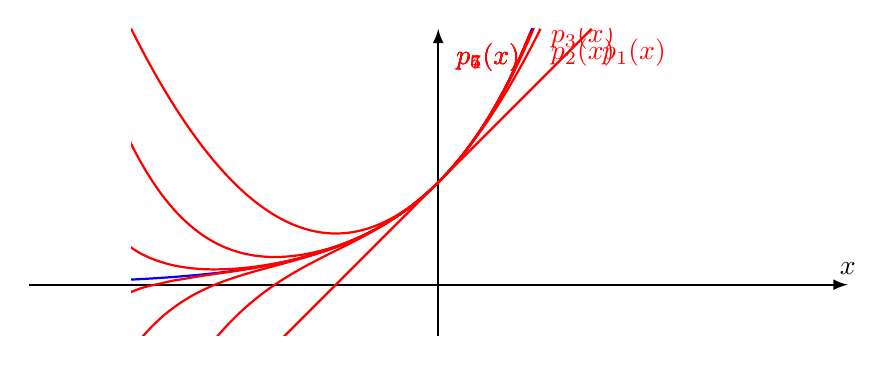
\begin{tikzpicture}[>=latex,thick,scale=1.3]
      \draw[->] (-4.0, 0.0) -- (4.0,0.0) coordinate[label=$x$];
      \draw[->] ( 0.0,-0.5) -- (0.0,2.5);
      \clip (-3,-0.5) rectangle (3,2.5);
      \draw[domain=-4:1, samples=50, smooth, blue]
        plot ({\x}, {exp(\x)})
        node[above right] {$\exp(x)$};
      \uncover<1>{
      \draw[domain=-4:1.5, samples=10, smooth, red]
        plot ({\x}, {1 + \x})
        node[below right] {$p_1(x)$};}
      \uncover<2>{
      \draw[domain=-4:1, samples=50, smooth, red]
        plot ({\x}, {1 + \x + \x*\x/2})
        node[below right] {$p_2(x)$};}
      \uncover<3>{
      \draw[domain=-4:1, samples=50, smooth, red]
        plot ({\x}, {1 + \x + \x*\x/2 + \x*\x*\x/6})
        node[below right] {$p_3(x)$};}
      \uncover<4>{
      \draw[domain=-4:0.9, samples=50, smooth, red]
        plot ({\x}, {1 + \x + \x*\x/2 + \x*\x*\x/6 + \x*\x*\x*\x/24})
        node[below left] {$p_4(x)$};}
      \uncover<5>{
      \draw[domain=-4:0.9, samples=50, smooth, red]
      plot ({\x}, {1 + \x + \x*\x/2 + \x*\x*\x/6 + \x*\x*\x*\x/24
        + \x*\x*\x*\x*\x/120})
      node[below left] {$p_5(x)$};}
      \uncover<6>{
      \draw[domain=-4:0.9, samples=50, smooth, red]
      plot ({\x}, {1 + \x + \x*\x/2 + \x*\x*\x/6 + \x*\x*\x*\x/24
        + \x*\x*\x*\x*\x/120
        + \x*\x*\x*\x*\x*\x/720})
      node[below left] {$p_6(x)$};}
      \uncover<7>{
      \draw[domain=-4:0.9, samples=50, smooth, red]
      plot ({\x}, {1 + \x + \x*\x/2 + \x*\x*\x/6 + \x*\x*\x*\x/24
        + \x*\x*\x*\x*\x/120
        + \x*\x*\x*\x*\x*\x/720
        + \x*\x*\x*\x*\x*\x*\x/5040})
      node[below left] {$p_7(x)$};}
    \end{tikzpicture}
  \end{center}
\end{frame}

\egroup
